\section{Qualità di Processo}

\subsection{Introduzione}

Per garantire la qualità del prodotto finale, si è deciso di fare uso del metodo del PDCA  e di fare riferimento allo standard \glock{ISO/IEC:9126} per la definizione delle caratteristiche di qualità del prodotto.
Attraverso questo metodo e quelle caratteristiche è possibile garantire un miglioramento continuo con un focus sull'ottenimento di un prodotto di qualità.

Nello svolgimento del progetto, i processi fanno uso di criteri di qualità, attraverso i quali è possibile perseguire un miglioramento continuo che porti alla più completa soddisfazione di questi criteri. In questo progetto, si è scelto di fare uso del metodo PDCA e dello standard ISO/IEC 15504 (SPICE). Attraverso \glock{PDCA} e \glock{SPICE}, è possibile garantire uno svolgimento dei processi che tendono, attraverso l'esperienza, a migliorarsi e ad assicurare al cliente l'ottenimento di un prodotto di qualità.
In questa sezione si espongono i livelli di qualità accettabili e ottimali sulla base delle metriche scelte all'interno del documento \dext{Norme di Progetto v1.0.0}.

\subsection{Monitoraggio dei Processi}

I processi monitorati con delle metriche precise di qualità sono i seguenti:

\begin{itemize}
	\item Gestione delle Spese/Risorse (Piano di Progetto);
	\item Gestione dei Rischi.
\end{itemize}

	\subsubsection{QPC-1 Gestione delle Spese}

		Il processo di gestione delle risorse si riserva di gestire la copertura delle risorse disponibili e delle attività schedulate all'interno del \dext{Piano di Progetto v1.0.0}. 
		Di seguito vengono esposte le metriche utilizzate, che possono essere visionate all'interno del documento \dext{Norme di Progetto v1.0.0}.

		\paragraph{Metriche utilizzate}

			\begin{itemize}
				\item QM-PC-PNF01 Budgeted Cost of Work Scheduled (BCWS)
				\item QM-PC-PNF02 Actual Cost of Work Performed (ACWP)
				\item QM-PC-PNF03 Budgeted Cost of Work Performed (BCWP)
				\item QM-PC-PNF04 Cost Variance (CV)
				\item QM-PC-PNF05 Schedule Variance (SV)
			\end{itemize}

		\paragraph{Indici di Qualità}

			\begin{center}
				\rowcolors{2}{white}{lightest-grayest}
				\begin{longtable}{|c|c|c|}
				\hline
				\rowcolor{lighter-grayer}
				\textbf{ID Metrica} & \textbf{Valore Preferibile} & \textbf{Valore Accettabile}\\
				\hline
				\endfirsthead
				\hline
				BCWS & // & // \\
				\hline
				ACWP & // & // \\
				\hline
				BCWP & // & // \\
				\hline
				CV & \(0\%\) & \(\ge -5\%\) \\
				\hline
				SV & \(0\%\) & \(\ge -5\%\) \\
				\hline
				\caption{Indici di qualità per le metriche per la Gestione delle Risorse}
				\end{longtable}
			\end{center}

	\subsubsection{QPC-2 Gestione dei Rischi}

		Il processo di gestione della qualità monitora l'adempimento delle metriche definite per ogni processo.
		Per ogni fase del progetto si eseguirà un'analisi "istantanea" della situazione corrente, con successivo richiamo per non adempimento a qualche metrica prescritta.
		Di seguito vengono esposte le metriche utilizzate, che possono essere visionate all'interno del documento \dext{Norme di Progetto v1.0.0}.

		\paragraph{Metriche utilizzate}
			\begin{itemize}
				\item QM-PD-SVL01 Percentuale requisiti soddisfatti (PRS) 
			\end{itemize}
			
		\paragraph{Indici di Qualità}
			\begin{center}
				\rowcolors{2}{white}{lightest-grayest}
				\begin{longtable}{|c|c|c|}
				\hline
				\rowcolor{lighter-grayer}
				\textbf{Metrica} & \textbf{Valore Preferibile} & \textbf{Valore Accettabile}\\
				\hline
				\endfirsthead
				\hline
				PRS & 0\% & 5\% \\
				\hline
				\caption{Indici di qualità per le metriche per la Gestione della Qualità}
				\end{longtable}
			\end{center}

			
			Di seguito il grafico che rappresenta la percentuale di violazioni delle metriche definite nelle \dext{Norme di Progetto}:
			
			\begin{figure}[H]
				\centering
				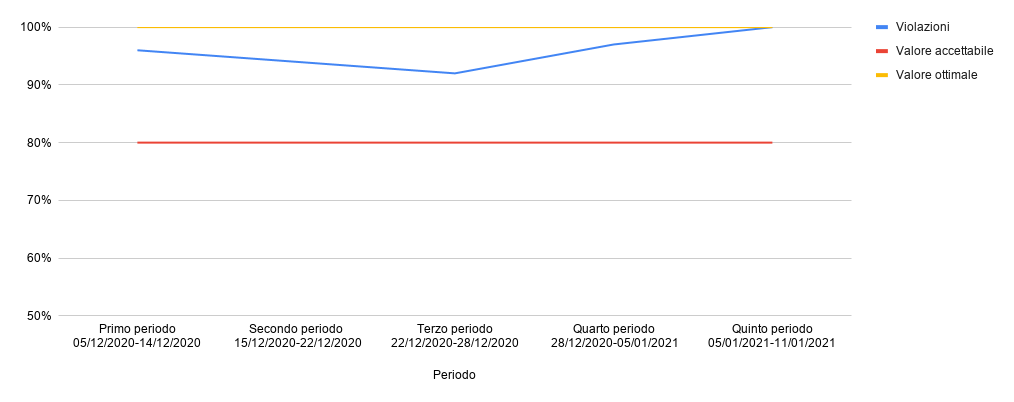
\includegraphics[width=0.9\linewidth]{./res/images/violazioni.png}
				\caption{Grafico periodo/ivolazione nel periodo di Analisi dei Requisiti}
				\label{fig:Grafico violazioni periodo di Analisi dei Requisiti}
			\end{figure}
			
			
			
			
			
			
			
			
			
			
			
			
			
			
			
			
			
			
			
			
			
	
	
	
	
	
	
	
	\subsubsection{QPC-2 Gestione della Qualità}

		Il processo di gestione dei rischi monitora la comparsa di nuovi rischi che possono avvenire durante le fasi del progetto.
		Per ogni fase del progetto si eseguirà una relativa analisi retrospettiva dei rischi precedentemente segnalati e, in caso di nuovi rischi, si cercherà di risolverli nel minor tempo possibile.
		Di seguito vengono esposte le metriche utilizzate, che possono essere visionate all'interno del documento \dext{Norme di Progetto v1.0.0}.

		\paragraph{Metriche utilizzate}
			\begin{itemize}
				\item QM-PC-PNF06 Unbudgeted Risks (UR)
			\end{itemize}
			
		\paragraph{Indici di Qualità}
			\begin{center}
				\rowcolors{2}{white}{lightest-grayest}
				\begin{longtable}{|c|c|c|}
				\hline
				\rowcolor{lighter-grayer}
				\textbf{ID Metrica} & \textbf{Valore Preferibile} & \textbf{Valore Accettabile}\\
				\hline
				\endfirsthead
				\hline
				UR & 0 rischi & 5 rischi \\
				\hline
				\caption{Indici di qualità per le metriche per la Gestione delle Risorse}
				\end{longtable}
			\end{center}

			
			Di seguito il grafico che rappresenta i rischi non preventivati per il periodo di Analisi dei Requisiti:
			
			\begin{figure}[H]
				\centering
				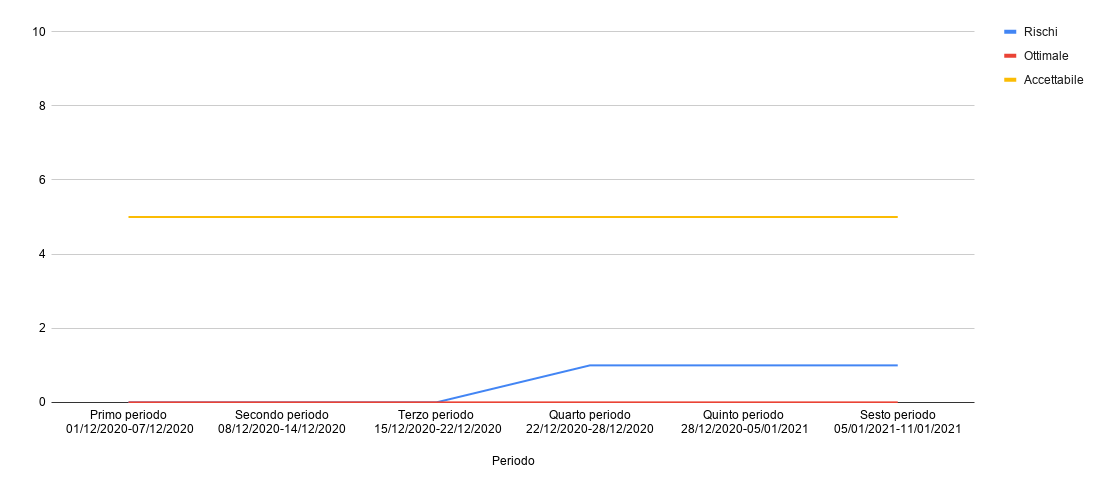
\includegraphics[width=0.9\linewidth]{./res/images/rischi.png}
				\caption{Grafico periodo/rischio nel periodo di Analisi dei Requisiti}
				\label{fig:Grafico rischi periodo di Analisi dei Requisiti}
			\end{figure}

